\documentclass[onecolumn, draftclsnofoot,10pt, compsoc]{IEEEtran}

\usepackage{float}
\usepackage{graphicx}
\usepackage{url}
\usepackage{setspace}
\usepackage{geometry}
\usepackage{listings}
\usepackage{color}
\usepackage{etoolbox}
\usepackage{pdflscape}

\patchcmd{\thebibliography}{\section*{\refname}}{}{}{}

\geometry{textheight=9.5in, textwidth=7in}

% 1. Fill in these details
\def \CapstoneTeamName{			              			 PlanteR-GB}
\def \CapstoneTeamNumber{					           			 Group 64}
\def \GroupMemberOne{				           				Austin Hodgin}
\def \GroupMemberTwo{				           				Travis Hodgin}
\def \GroupMemberThree{			            Maximillian Schmidt}
\def\GroupMemberFour{		        	               Zach Lerew}
\def \CapstoneProjectName{	      	    Winter is Coming...}
\def \CapstoneSponsorCompany{		    Oregon State University}
\def \CapstoneSponsorPerson{		 			  				 Victor Hsu}

% 2. Uncomment the appropriate line below so that the document type works
\def \DocType{		%Problem Statement
				%Requirements Document
				%Technology Review
				%Design Document
				%Fall Progress Report
				Spring Progress Report
				}

\newcommand{\NameSigPair}[1]{\par
\makebox[2.75in][r]{#1} \hfil 	\makebox[3.25in]{\makebox[2.25in]{\hrulefill} \hfill		\makebox[.75in]{\hrulefill}}
\par\vspace{-12pt} \textit{\tiny\noindent
\makebox[2.75in]{} \hfil		\makebox[3.25in]{\makebox[2.25in][r]{Signature} \hfill	\makebox[.75in][r]{Date}}}}
% 3. If the document is not to be signed, uncomment the RENEWcommand below
\renewcommand{\NameSigPair}[1]{#1}

%%%%%%%%%%%%%%%%%%%%%%%%%%%%%%%%%%%%%%%
\begin{document}
\begin{titlepage}
    \pagenumbering{gobble}
    \begin{singlespace}
    	%\includegraphics[height=4cm]{coe_v_spot1}
        \hfill

        % 4. If you have a logo, use this includegraphics command to put it on the coversheet.
        
\includegraphics[height=4cm]{logo.png}

        \par\vspace{.2in}
        \centering
        \scshape{
            \huge CS Capstone \DocType \par
            {\large\today}\par
            \vspace{.5in}
            \textbf{\Huge\CapstoneProjectName}\par

            %\vfill
						\vspace{1in}

            {\large Prepared for}\par
            \Huge \CapstoneSponsorCompany\par
            \vspace{5pt}
            {\Large\NameSigPair{\CapstoneSponsorPerson}\par}

						\vspace{1in}

            {\large Prepared by}\par
						{\huge \CapstoneTeamNumber}\par
            \CapstoneTeamName\par
            \vspace{5pt}

            {
							\Large
							\NameSigPair{\GroupMemberOne}\par
							\NameSigPair{\GroupMemberTwo}\par
							\NameSigPair{\GroupMemberThree}\par
							\NameSigPair{\GroupMemberFour}\par
            }

            \vspace{20pt}
        }
%\textbf{\textsuperscript{citation needed}}
				\newpage
        \begin{abstract}
				\noindent This document details what the team has accomplished for the final stage of the project.
				It covers the progress made on the bug fixing and polishing portion of the project,
				as well as problems we faced and the solutions implemented.
        \end{abstract}
    \end{singlespace}
\end{titlepage}

\newpage

\pagenumbering{arabic}
\tableofcontents
% 7. uncomment this (if applicable). Consider adding a page break.
%\listoffigures
%\listoftables
\clearpage
\singlespace

\newpage


% Syntax highlighting
\definecolor{mygreen}{rgb}{0,0.6,0}
\definecolor{mygray}{rgb}{0.5,0.5,0.5}
\definecolor{mymauve}{rgb}{0.58,0,0.82}

\lstset{
  backgroundcolor=\color{white},   % choose the background color
  basicstyle=\footnotesize,        % size of fonts used for the code
  breaklines=true,                 % automatic line breaking only at whitespace
  captionpos=b,                    % sets the caption-position to bottom
  commentstyle=\color{mygreen},    % comment style
  escapeinside={\%*}{*)},          % if you want to add LaTeX within your code
  keywordstyle=\color{blue},       % keyword style
  stringstyle=\color{mymauve},     % string literal style
	frame = single,                  % code framing
}


%%%%%%%%%%%%%%%%%%%%%%% NOTES %%%%%%%%%%%%%%%%%%%%%%%
%
%%%%%%%%%%%%%%%%%%%%%%%%%%%%%%%%%%%%%%%%%%%%%%%%%%%%%


	% Introduction
	\section{Purpose}
	The PlanteR-GB project is a configurable LED strip control system run by microcontrollers.
	The system intends to make growing plants easy and configurable by giving the user control over the state of every LED connected to the system.
	Through a local web interface, the system groups LEDs across multiple light strips into zones.
	Zones set the color, intensity, and power state of their LEDs based on a configurable schedule.
	Existing plant lighting systems offer little to no configuration options and cost between \$70 and \$100. \cite{expensive1} \cite{expensive2} \cite{expensive3}
	Our team is building an LED plant growing system from the ground up to offer configuration options and affordability.
	The trade off made for a lower price is more involvement during setup. Our team intends to release the project as open source software for the DIY community.
	Initially the project will require users to purchase the specific micro controllers used by the system, flash the control software, and wire the system together.
	Our stretch goals include purchasable kits which include all of the necessary parts and instructions to build the system for yourself, and possibly custom enclosures that are sold as pre-made working systems.

	\section{Goals}
	The PlanteR-GB lighting system will allow users to change individual LEDs to a specific color and intensity at any time throughout the day or week.
	LEDs on up to twenty light strips can be grouped into zones and controlled on a schedule with a local web interface.
	The 1.0 version of the project will have thorough testing and very few bugs. Some minor improvements and tweaks will be made throughout the process,
	but most of the effort between Beta and Release is testing and bug fixing.

	\section{Status}
	The project is now in a release state. The team's definition of a release state is the successful completion of all system requirements.
	\\
	The Internal State, API, and DataParser have all been thoroughly unit tested, and a large handful of bugs have been found and fixed because of it.
	\begin{center}
		\begin{figure}[H]
			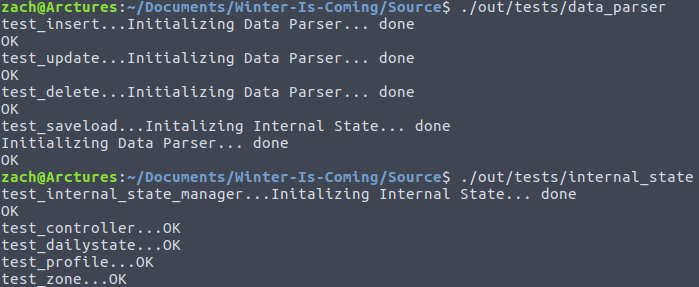
\includegraphics[width=\linewidth]{tests/internal_state_data_parser_tests.png}
			\caption{Passing internal state and data parser tests}
			\label{fig:isdpTests}
		\end{figure}
	\end{center}

	\begin{center}
		\begin{figure}[H]
			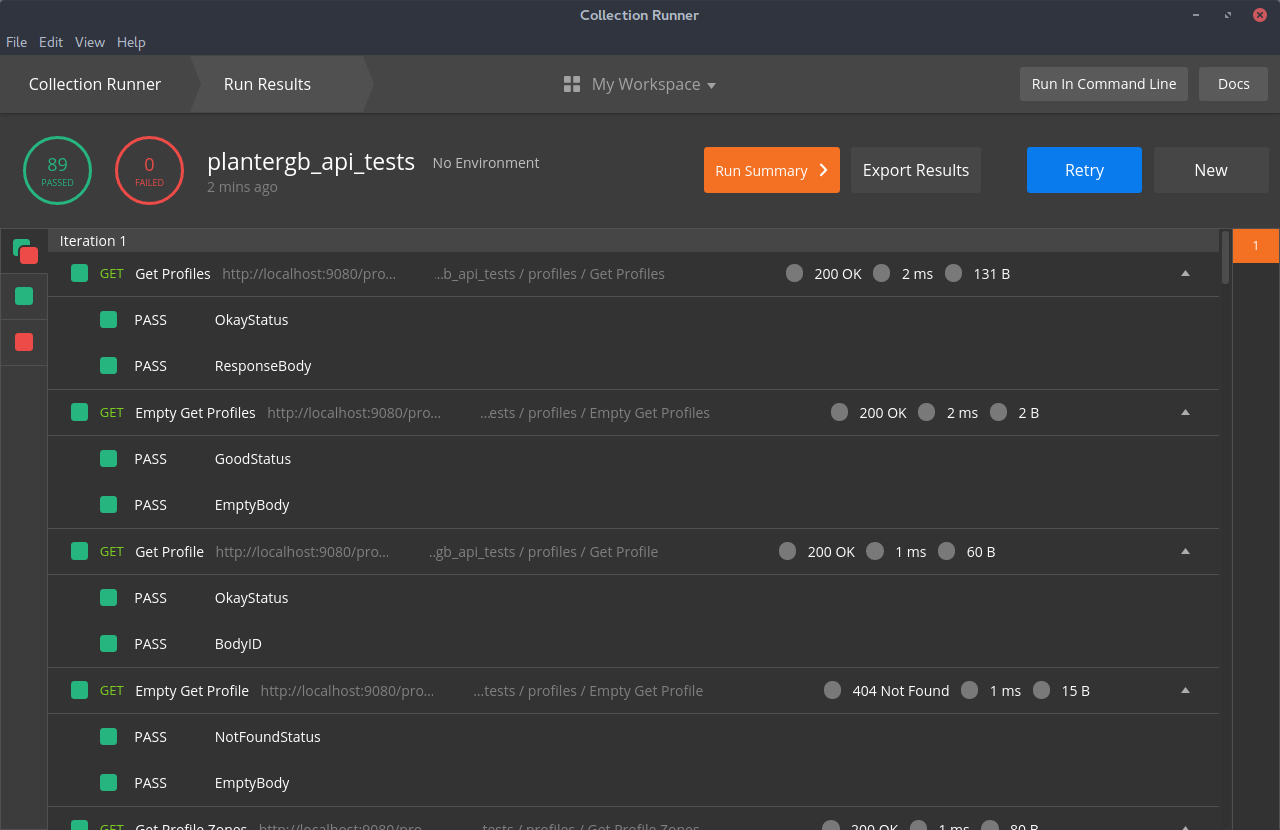
\includegraphics[width=\linewidth]{tests/api_tests.png}
			\caption{Passing API tests using postman}
			\label{fig:apiTests}
		\end{figure}
	\end{center}
	\\
	The State Composer remains untested, and currently still has the bug from ALPHA that turned random lights to random colors. However, this bug only
	occurs for the system with three strips at full brightness.
	\\
	The Site has basic unit testing completed, but needs more work when it comes to confirming that the pages are rendering data correctly.
	It has also had a variety of minor improvements and tweaks, and is in very good shape.

	\section{Problems}
	\subsection{Random LEDs changing colors, entire strips occasionally denying input}
    	This problem has plagued us since the first time we got LEDs to work.
		At first it was due to using the UART serial protocol, but that was replaced with I2C which allows for complicated addressing over a single bus.
		After that, we implemented a system that would store the state active for every zone in the system.
		In order to send serial data, the state composer first checks to see if the state has changed for each zone.
		This reduced the chances of the serial bus becoming saturated and corrupting data.
		The last change was to open the I2C bus before writing to it, and close it when done. This added extra work for each write, but also eliminated some issues.
		The system now works perfectly with two controllers. However, only one controller has an LED strip of 60, and it is set to 20 percent brightness.
		We have still been seeing issues when using a system with an advanced power supply running three controllers and three LED strips at full brightness.
  	\subsubsection{Solution}
		We have found solutions to get at least one variation of our system working, that is with a single strip of lights at 20 percent brightness.
		However, we have not yet found a solution to the three strips problem. It is a very difficult one to debug because it is intermittent and random.


	\section{Remaining work}
	All required goals were met.
	During the remaining week some work may continue on stretch goals such as Site improvements, custom enclosure modeling, and more thorough testing.


	\section{References}
			\begingroup
				\renewcommand{\addcontentsline}[3]{}% Remove functionality of \addcontentsline
				\renewcommand{\section}[2]{}% Remove functionality of \section
				%\cite[Sec 3.8]{sourceName}
				\bibliography{ref}
				\bibliographystyle{IEEEtran}
			\endgroup
\end{document}
